% 例 3：等边 △ABC 外一点 D，绕 A 逆时针 60° 把 △ABD 转到 △ACD'
\documentclass[tikz,border=4pt]{standalone}
\usepackage{ctex}
\usepackage{amsmath}
\usetikzlibrary{calc, decorations.markings, arrows.meta}
\begin{document}
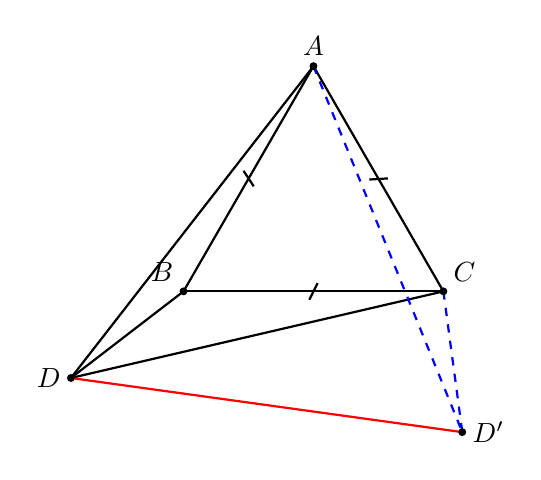
\begin{tikzpicture}[scale=1.1, thick,
  tickone/.style={postaction={decorate, decoration={markings,
    mark=at position 0.5 with {\draw (-1.5pt,-3pt) -- (1.5pt,3pt);}}}}]
  % 等边三角形 ABC，A 顶
  \coordinate (A) at (0, 2.6);
  \coordinate (B) at (-1.5, 0);
  \coordinate (C) at (1.5, 0);
  % D 在外面（B 左下）
  \coordinate (D) at (-2.8, -1.0);
  % 把 △ABD 绕 A 逆时针 60°：B 转到 C，D 转到 D'
  % D-A = (-2.8, -3.6) ; 旋转60°逆：x'= x cos60 - y sin60 = -2.8*0.5 - (-3.6)*0.866=-1.4+3.118=1.718
  % y' = x sin60+y cos60 = -2.8*0.866+(-3.6)*0.5=-2.4248-1.8=-4.2248
  % D' = A + (1.718, -4.225) = (1.718, 2.6 - 4.225)=(1.718,-1.625)
  \coordinate (Dp) at (1.718, -1.625);

  \draw[tickone] (A) -- (B);
  \draw[tickone] (B) -- (C);
  \draw[tickone] (C) -- (A);
  \draw (A) -- (D);
  \draw (B) -- (D);
  \draw (C) -- (D);
  % 旋转后
  \draw[blue, dashed] (A) -- (Dp);
  \draw[blue, dashed] (C) -- (Dp);
  % DD' 红
  \draw[red, thick] (D) -- (Dp);

  \fill (A) circle (1.3pt); \fill (B) circle (1.3pt);
  \fill (C) circle (1.3pt); \fill (D) circle (1.3pt); \fill (Dp) circle (1.3pt);
  \node[above] at (A) {$A$};
  \node[above left] at (B) {$B$};
  \node[above right] at (C) {$C$};
  \node[left] at (D) {$D$};
  \node[right] at (Dp) {$D'$};
\end{tikzpicture}
\end{document}
